\documentclass[10 pt]{article}
\usepackage{graphicx}
\pagestyle{plain}
\usepackage[OT4]{polski}
\usepackage[utf8]{inputenc}
\title{Sprawozdzanie 6 \\ \emph{\textbf{Porównanie wyszukiwania elementu w strukturze drzewiastej, tabilcy asocjacyjnej oraz tablicy z haszowaniem}}}
\author{Paweł Żurek 200404}
\date{22.04.2014}
\begin{document}
\tableofcontents
\maketitle
\section{Wstęp}
Program porównuje czas wyszukiwania elementu w 3 różnych strukturach :
\begin{itemize}
\item Drzewo
\item Tablica asocjacyjna
\item Tablica z haszowaniem
\end{itemize}

\section{Krótki opis programu}
Program wczytuje plik z 100 elementami ( początek Inwokacji ). Dodaje do struktury wszystkie 100 słów a następnie wyszukuje każde z osobna.

\section{Wynik:}

\paragraph{Dane zilustrowane w formie wykresu ( dane oraz wykres dostępne w pliku wynik.xlsx ) \\}
\begin{center}
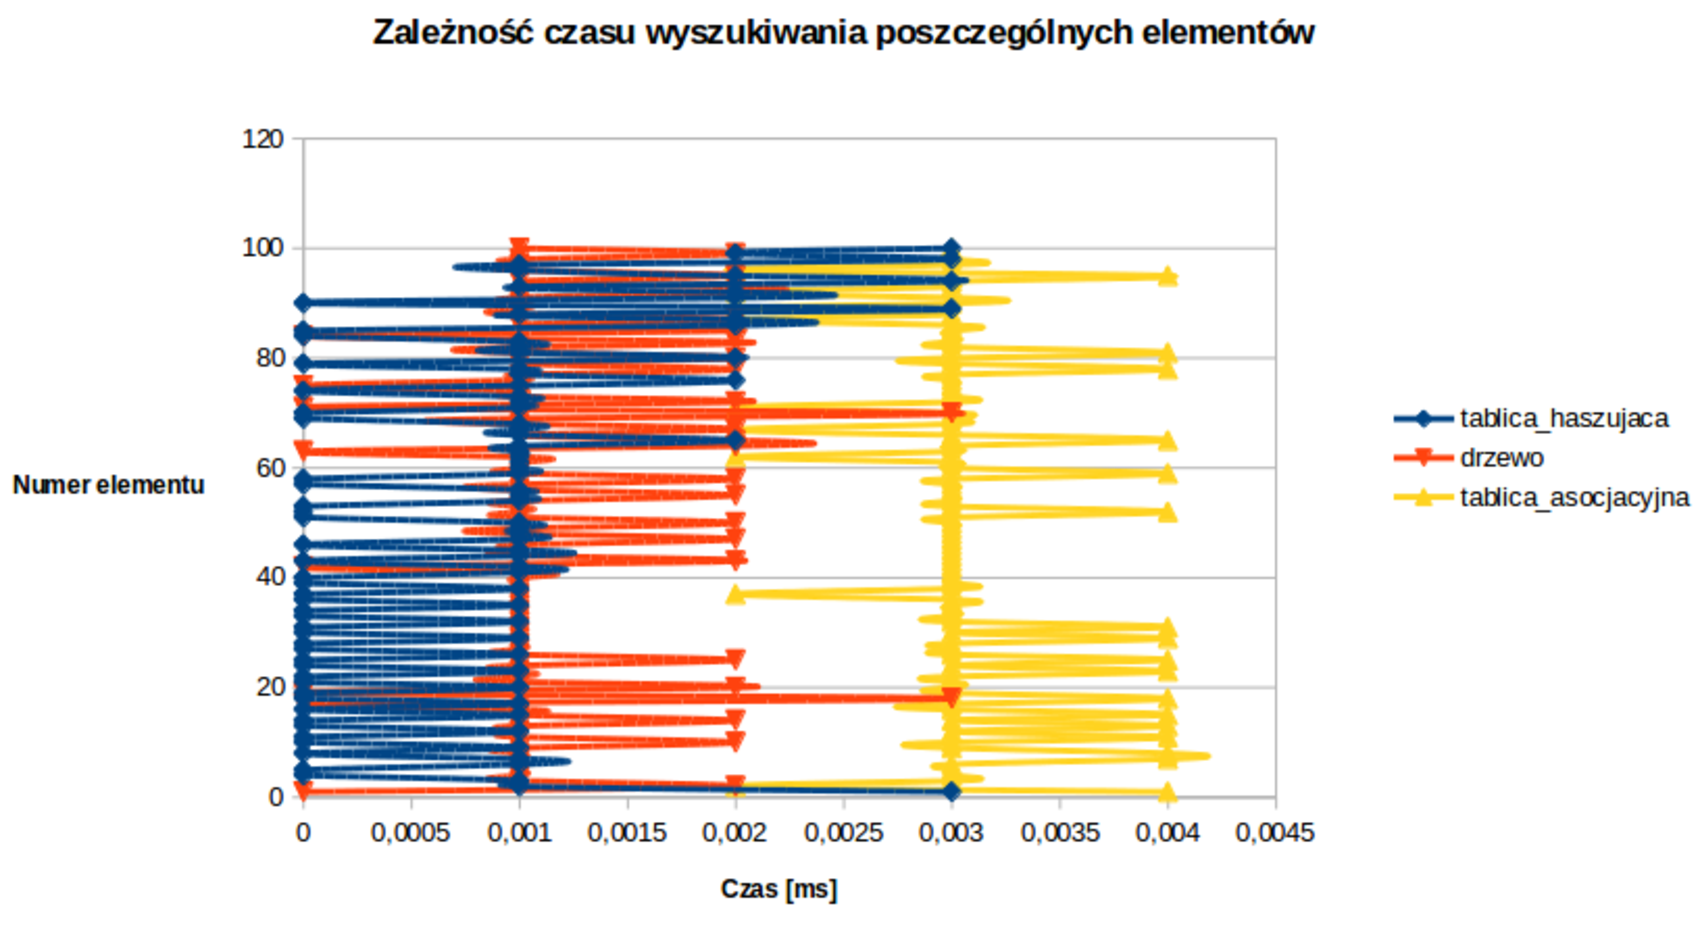
\includegraphics[scale=0.5]{wykres.pdf}
\end{center}

\section{Wnioski:}
\begin{itemize}
\item Program działa poprawnie
\item Z wykresu jasno widać, że najszybszą strukturą okazała się tablica z haszowaniem. Jest to prawdopodobnie dobry wynik, poniważ algorytm tablicy z haszowaniem jest najdokładniejszy. Tzn dla większość elementów jest wyszukiwana w czasie O(1)
\item Ciężko jednak stwierdzić jasno, która struktura jest najszybsza, ponieważ wyniki te są tylko dla 100 elementów
\item Wyniki można zinterpretować następująco : 
\begin{itemize}
\item najszybszą metodą jest odwoływanie się do elementu bezpośrednio poprzez jego indeks
\item drugą najszybszą metodą okazała się rekurencja
\item najwolniejszą metodą okazało się wyszukiwanie iteracyjne
\end{itemize}

\end{itemize}

\end{document}